\chapter{Web Server - Design of Experiment}
Obiettivo: Design an experiment to study the impact of two factors (intensity and page type) on the response time
\section{Design}
Descrizione fattori scelti repliche ecc ...
collezionamento response time medio
\section{Analisi}
Il design oggetto di studio è un \textit{Two-factor Full Factorial Design con repliche}.
I fattori che lo interessano sono categorici, quindi possono assumere solo valori finiti. 
\\La seguente tabella descrive i tempi medi di risposta ottenuti in funzione delle combinazioni dei fattori e delle repliche:
\\
\begin{table*}[h]
	\begin{center}
		\begin{tabular}{|c|c|c|c|c|}
			\hline
			Intensity & Small & Small-Medium & Meduim-Large & Large\\
			\hline
			\rule[-4mm]{0mm}{0.5cm}
			1500 & 5,2082 & 23,5713 & 42,0207 & 78,6531\\
			\rule[-4mm]{0mm}{0.5cm}
			& 5,7017 & 16,3747 & 32,3323 & 54,5792\\
			\rule[-4mm]{0mm}{0.5cm}
			& 5,4777 & 19,1214 & 32,6010 & 39,0433\\
			\rule[-4mm]{0mm}{0.5cm}
			& 5,9955 & 14,0742 & 36,6634 & 47,6427\\	
			\rule[-4mm]{0mm}{0.5cm}
			& 5,1065 & 16,8909 & 41,6693 & 55,1706\\ 
			\hline
			\rule[-0.5cm]{0mm}{0.5cm}
			4500 & 5,1412 & 15,4733 & 380,9312 & 552,1893\\
			\rule[-0.5cm]{0mm}{0.5cm}
			& 4,5569 & 18,6695 & 379,4760 & 538,0078\\
			\rule[-0.5cm]{0mm}{0.5cm}
			& 4,6629 & 23,1843 & 375,8755 & 539,3999\\
			\rule[-0.5cm]{0mm}{0.5cm}
			& 4,4400 & 21,3396 & 366,9233 & 575,0426\\	
			\rule[-0.5cm]{0mm}{0.5cm}
			& 4,3709 & 20,0086 & 368,5614 & 541,5188\\
			\hline
		\end{tabular}
	\end{center}
\end{table*}
\\
\\
Vedere se aggiungere :
\\Equazione modello
\\Computation of Effects
\\Interactions
\\Computation of Errors
\subsection{Importanza - Allocation of Variation}
L' \textit{importanza} di un fattore viene misurata in base alla porzione di \textbf{variazione totale} che esso riesce a spiegare.
\\Quest'ultima è espressa tramite la Sum of Squares Total o \textit{SST} la quale ci fornisce informazioni circa quanto i dati ottenuti si discostano dal loro valore medio.
\begin{equation*}
	SST = \sum_{i = 1}^{n}{({y_i} - \overline{y})^2}
\end{equation*}
In particolare la variazione totale può essere anche vista come somma delle variazioni spiegate dai fattori, dalle loro interazioni e dall'errore commesso:
\\\textbf{SST = {SSA + SSB + SSAB + SSE}}.
\\La percentuale di variazione spiegata dal fattore A ad esempio è : \textbf{A = (SSA/SST)*100}.
\\
Queste informazioni possono essere agevolmente ottenute in \textit{JMP}, operando sulla tabella che caratterizza il design in questione, analizzando le sezioni:
\begin{enumerate}
	\item \textit{Analisi della varianza}
	\item \textit{Test degli effetti}
\end{enumerate}
\subsubsection{Caso di Studio}
\begin{figure}[H]
	\subfigure{	
		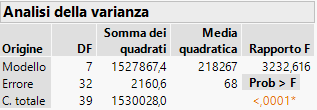
\includegraphics[width=0.50\textwidth]{img/hw4/AnalisiVarianza.png}}
	\subfigure{	
		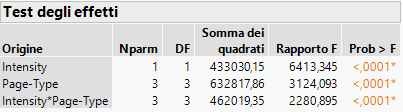
\includegraphics[width=0.50\textwidth]{img/hw4/TestEffetti.png}}
	\caption{\textit{Sum of Squares in JMP}}
\end{figure}
\begin{table*}[h]
	\begin{center}
		\begin{tabular}{|c|c|c|}
			\hline
			Component & Sum of Squares & \% Variation\\
			\hline
			 \rule[-4mm]{0mm}{0.5cm}
			 y - {$\overline{y}_...$}   	& 1530028,0		   & 100\\
			 \rule[-4mm]{0mm}{0.5cm}
			 Intensity (CTTs) 		  & 433030,15		   & 28,30\\
			 \rule[-4mm]{0mm}{0.5cm}
			 Page-Types 		  & 632817,86		   & 41,36\\
			 \rule[-4mm]{0mm}{0.5cm}
			 Interactions		  & 462019,35		   & 30,20\\
			 \rule[-4mm]{0mm}{0.5cm}
			 Errors 		  & 2160,6		   & 0,14\\
			\hline
		\end{tabular}
	\end{center}
\end{table*}
Osservando i risultati ottenuti notiamo che la percentuale maggiore di variazione la spiega il fattore \textit{Page Types}, con il 41,36\% della totale, seguito da \textit{Interazioni} e \textit{Intensità del carico} che ne spiegano una percentuale più o meno simile (rispettivamente 28,30\% e 30,20\%). Il restante 0,14\% è attribuita all'errore sperimentale.
\\
Tuttavia l'importanza non è un concetto statistico, dunque necessitiamo la valutazione di un altro parametro che invece lo è, la significatività.
Difatti può accadere che un fattore importante non sia significativo.
\subsection{Significatività - Analysis of Variance}
